\documentclass[a4paper]{article}
\usepackage[utf8]{inputenc}
\usepackage[T1]{fontenc}
\usepackage{graphicx}

\begin{document}

\title{Rapport projet couverture de graphe}
\author{Rémi Pérenne et Viktoriia Skrypnyk}
\maketitle

Q3.1 :
L'algorithme glouton n'est pas optimale car pour le graphe ci-dessous, il trouve \{0,4,5,6,7,8,9\} comme couverture alors que la couverture minimale est \{1,2,3\}. Il n'est donc pas 0.5-approché.

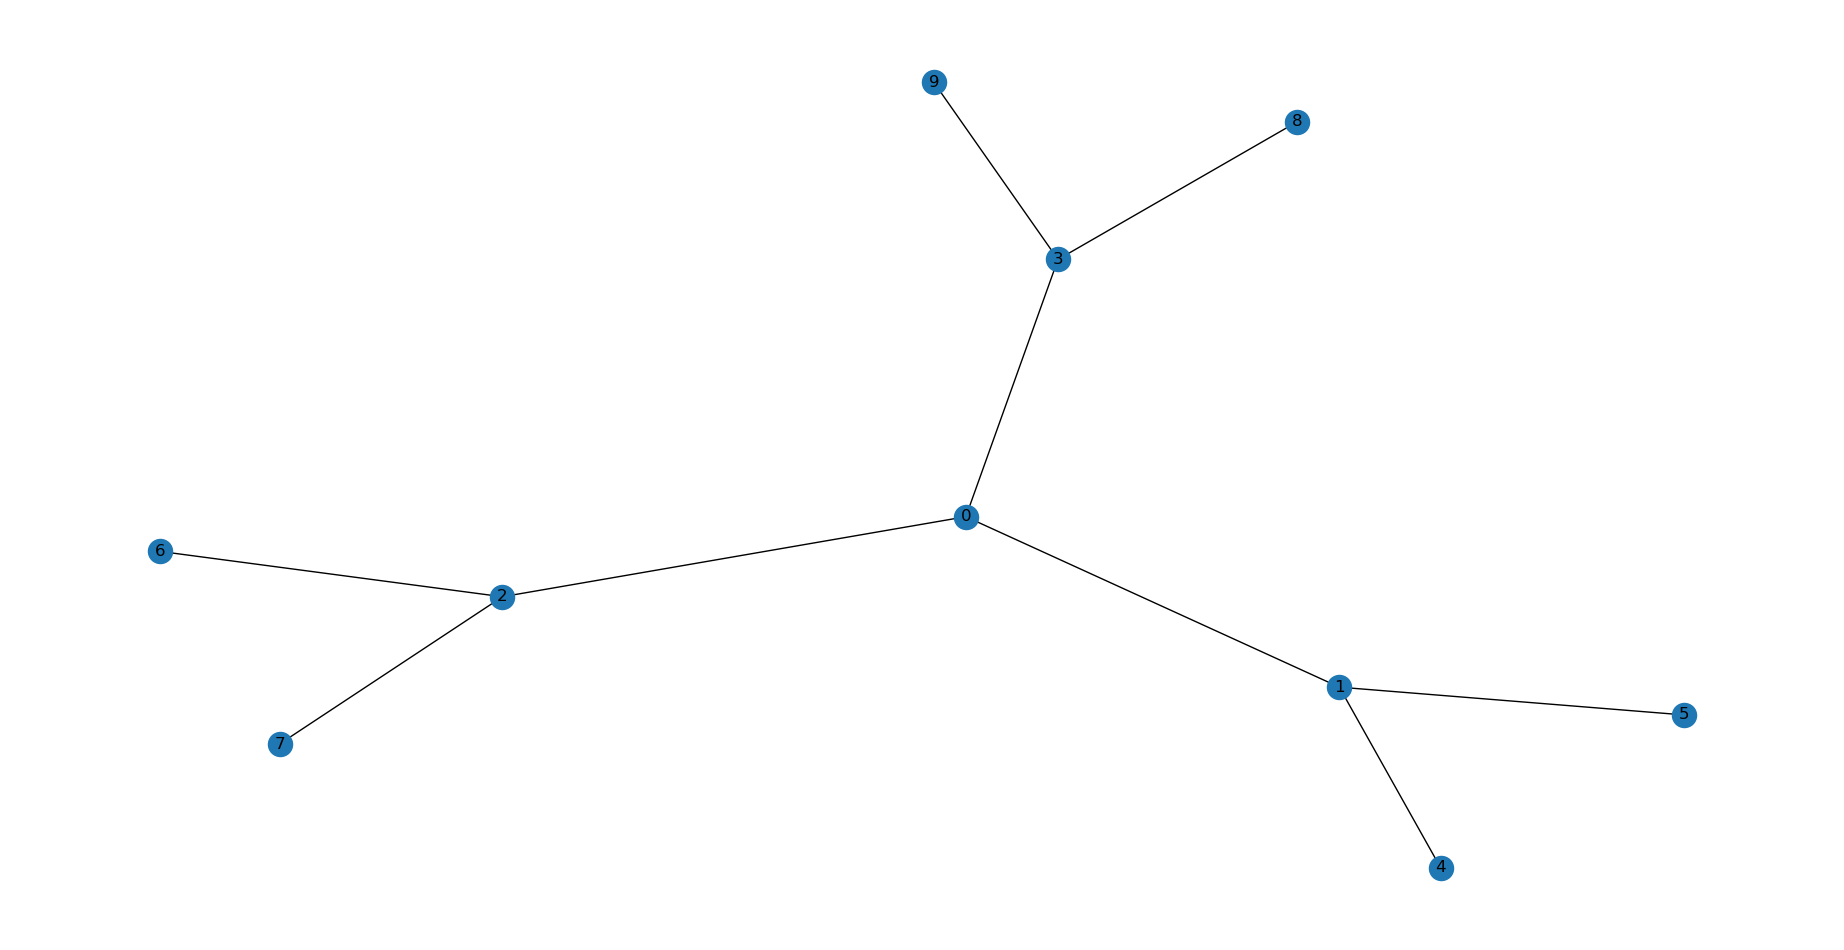
\includegraphics[scale=0.3]{"./graphe_q31.png"}

Q3.2 :
Voilà des graphiques permettant de comparer les 2 méthodes d'approximation. On peut voir que l'algorithme glouton donne sur les exemples des resultats similaire à la couverture minimale (calculée à l'aide d'un algorithme tiré des questions suivantes). L'algorithme de couplage quand à lui donne effectivement des ensembles d'aretes dont le cardinal est à peu près la moitié du cardinal d'une couverture minimale. On voit aussi que l'algorithme glouton prend bien plus de temps que l'algorithme de couplage pour s'executer. Ces observations sont vraies pour toutes les valeurs de $p$.

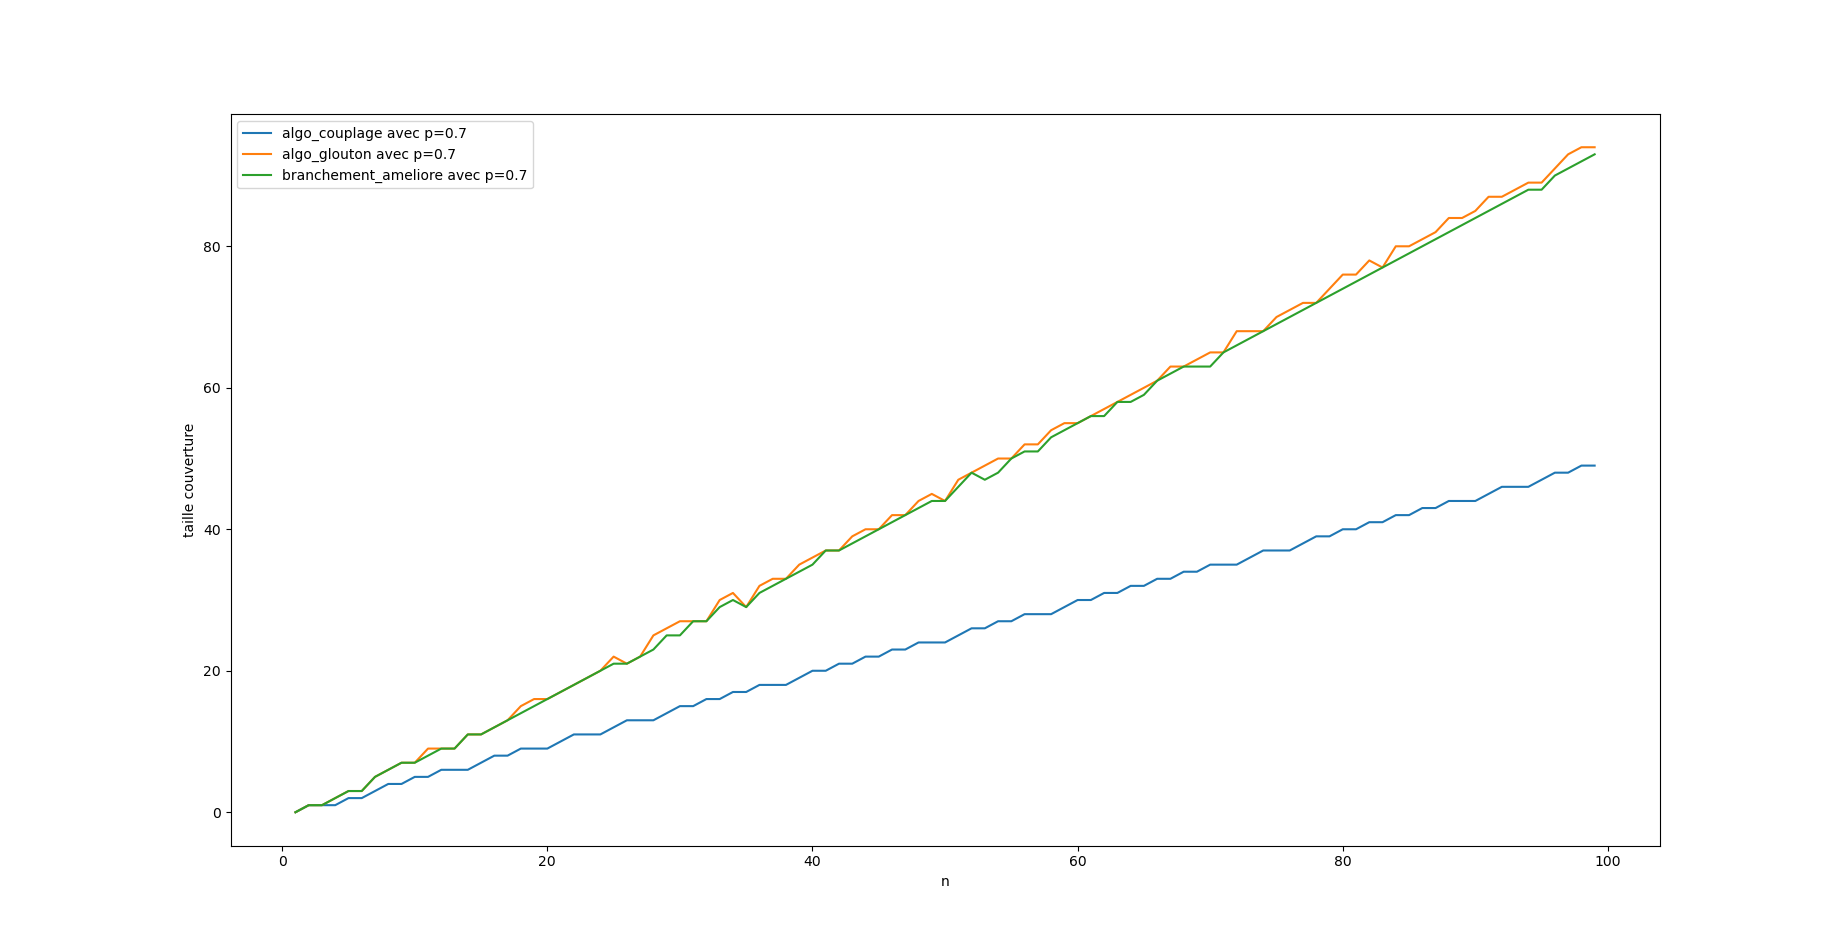
\includegraphics[scale=0.3]{"./comparaison_approximation_p07.png"}
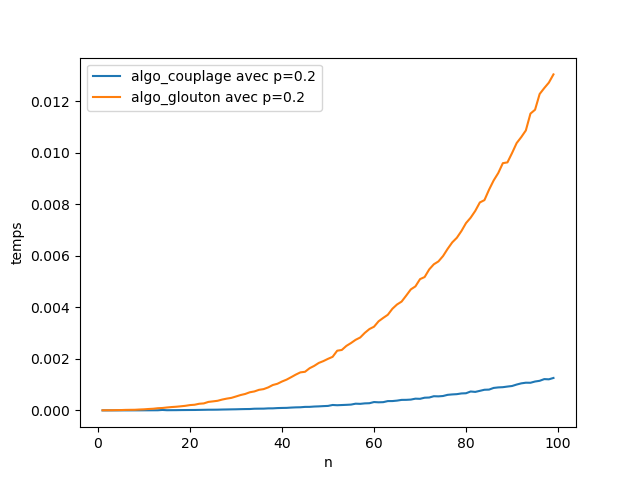
\includegraphics[scale=0.8]{"./comparaison_temps_approxs_p02.png"}

Q3.3 :
Soit $n$ un entier. Considérons le graphe $G_n$ définit par : $S=\{0,1,...,n + n(n-2)\}$ et $A=\{(0,i), \ \forall i \in [1;n]\} \bigcup ( \bigcup_{i=1}^{i=n} \{(i,j), \forall j \in [n+1+(i-1)(n-2):n+1+i(n-2)-1]\} )$. L'algorithme glouton commence par prendre le sommet $0$ puis il prend tout les sommets de $n+1$ à $n+n(n-2)$. Alors que la solution optimale est de prendre les sommets $1$ à $n$. Le rapport est donc de l'ordre de $n$ ce qui montre que l'algorithme glouton n'est pas $r$ approché pour tout $r$ (il suffit de faire tendre $n$ vers l'infinie). \\

Q4.1.2 :
Voilà des graphiques permettant de tester le temps ainsi que le nombre de noeuds générés par l'algorithme de branchement. On constate effectivement une évolution exponentiel du nombre de noeuds et du temps pris pour executer la fonction en fonction du nombre de noeuds $n$ dans le graphe.

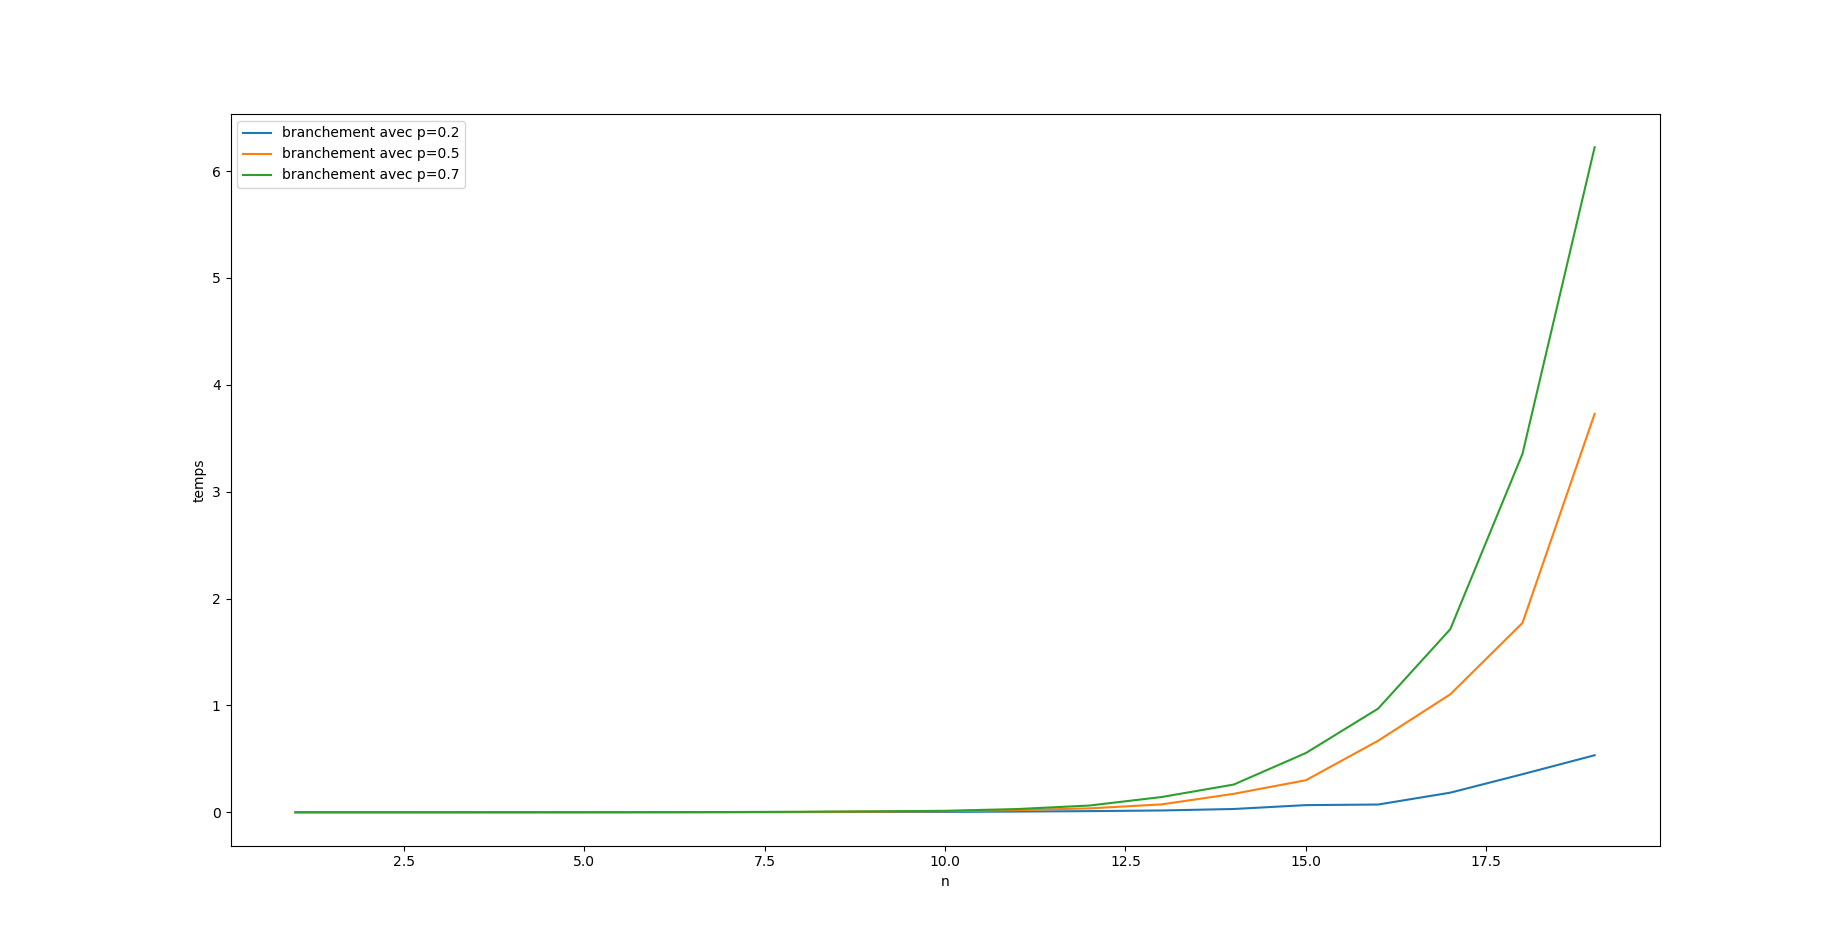
\includegraphics[scale=0.3]{"./test_branchement.png"}
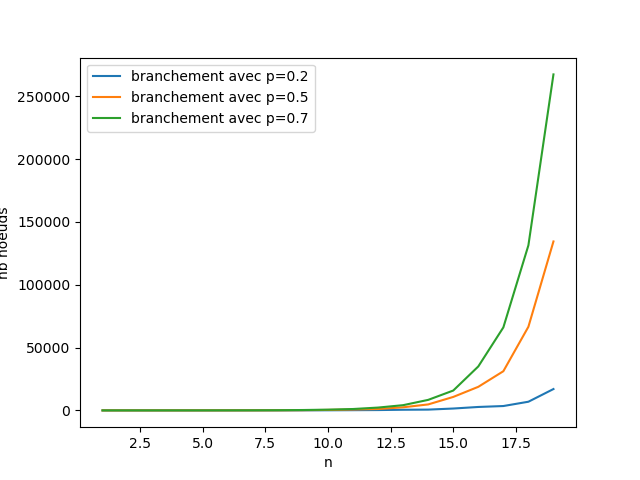
\includegraphics[scale=0.8]{"./test_nb_noeuds_branchement.png"}

Q4.2.1 : Pour la borne $b_1$, on sait qu'il y a $m$ aretes et que lorsque l'on prend un sommet on prend au plus $\Delta$ aretes ainsi il faut prendre au moins $ \lceil \frac{m}{\Delta} \rceil $ sommets pour prendre toutes les aretes (la partie entière suérieure est là car on ne peut prendre qu'un nombre entier d'aretes...

Pour la borne $b_2$, il faut prendre une des deux extremités de chaque arete du couplage dans une couverture. Mais les aretes du couplage ne partagent aucun sommet il faut donc prendre au moins $|M|$ sommets.

Pour la borne $b_3$ on note qu'il y a $|C|$ sommets dans la couverture et $n-|C|$ sommets qui ne sont pas dans la couverture. Ainsi,  $m \leq \frac{|C|(|C|-1)}{2} + (n-|C|)|C|$ (en effet, chaque sommet de $C$ est connecté à au plus tout les autres sommets du graphe et les sommets qui ne sont pas dans la couverture ne peuvent pas être lié entre eux sinon il y aurait des aretes non couvertes... la formule s'obtient ensuite par combinatoire). Les racines de $|C| + (1-2n)|C| + 2m = 0$ sont $|C| = \frac{2n - 1 \pm \sqrt{(2n-1)^2 - 8m}}{2}$ donc $m \leq \frac{|C|(|C|-1)}{2} + (n-|C|)|C| \iff |C| \in [\frac{2n - 1 - \sqrt{(2n-1)^2 - 8m}}{2};\frac{2n - 1 + \sqrt{(2n-1)^2 - 8m}}{2}]$ donc $|C| \leq \frac{2n - 1 + \sqrt{(2n-1)^2 - 8m}}{2}$ ce qui est le résultat attendu. \\

Q4.2.2 : 
Voilà des graphiques permettant de tester le temps ainsi que le nombre de noeuds générés par l'algorithme de branchement avec bornes. On constate effectivement une évolution exponentiel du nombre de noeuds et du temps pris pour executer la fonction en fonction du nombre de noeuds $n$ dans le graphe mais c'est bien plus rapide que sans les bornes !

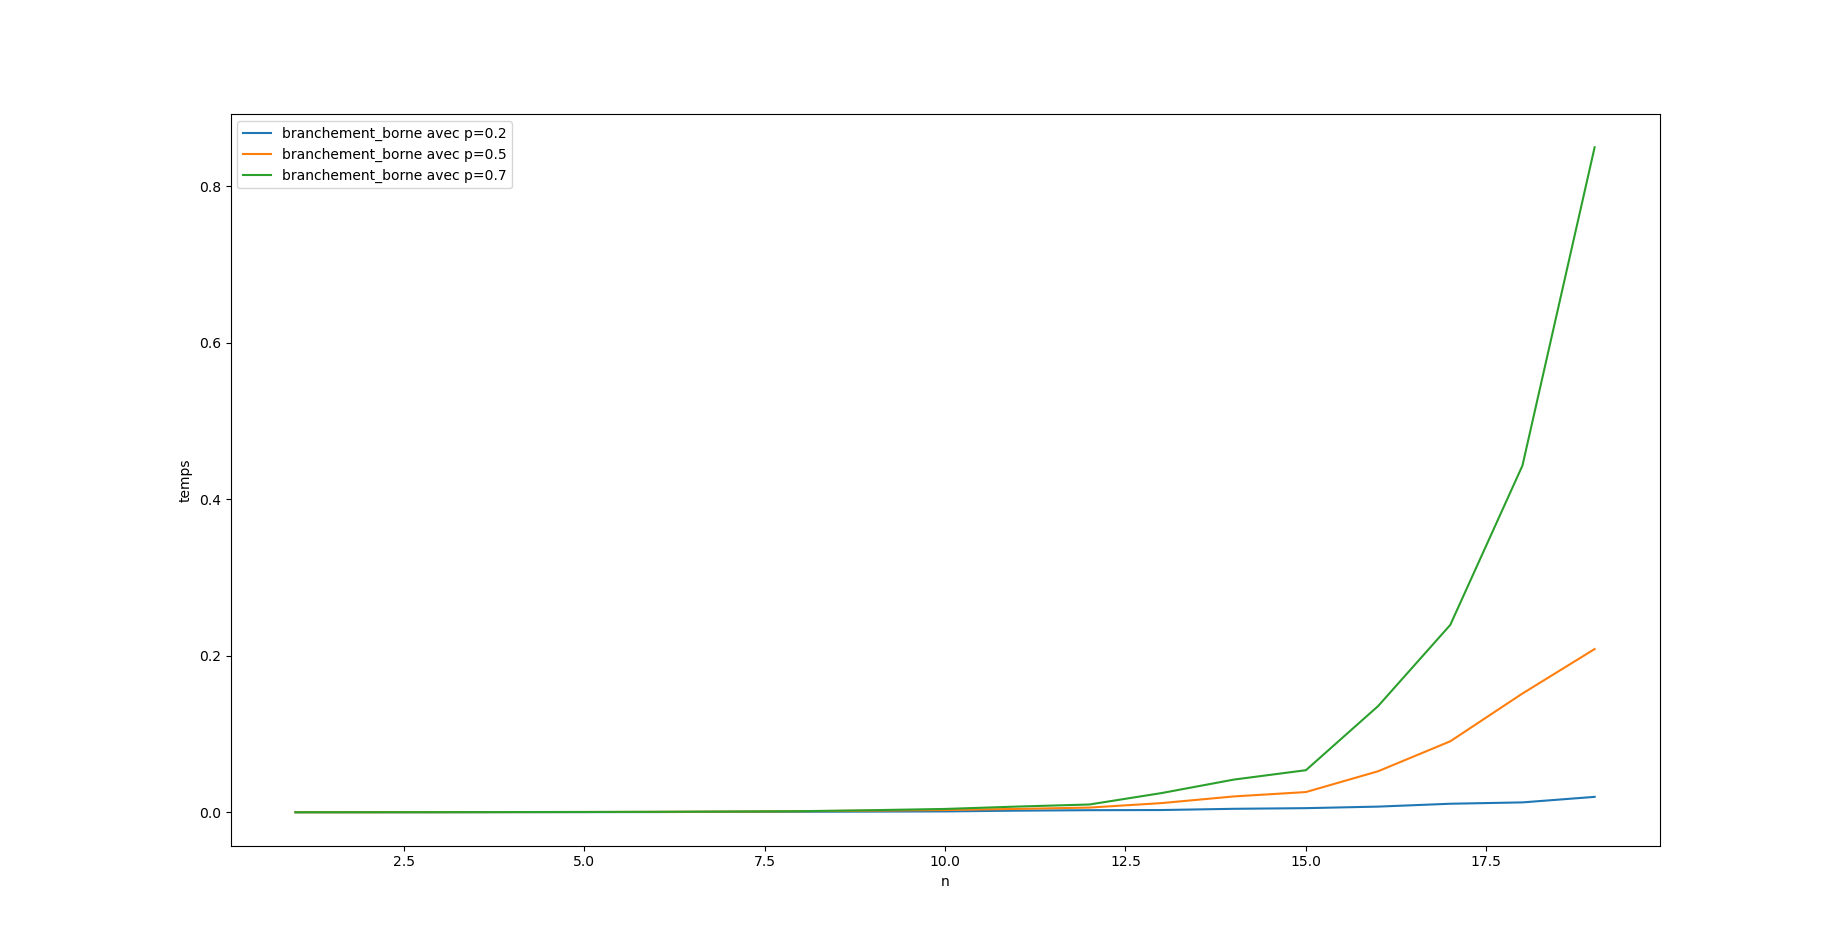
\includegraphics[scale=0.3]{"./test_branchement_borne.png"}
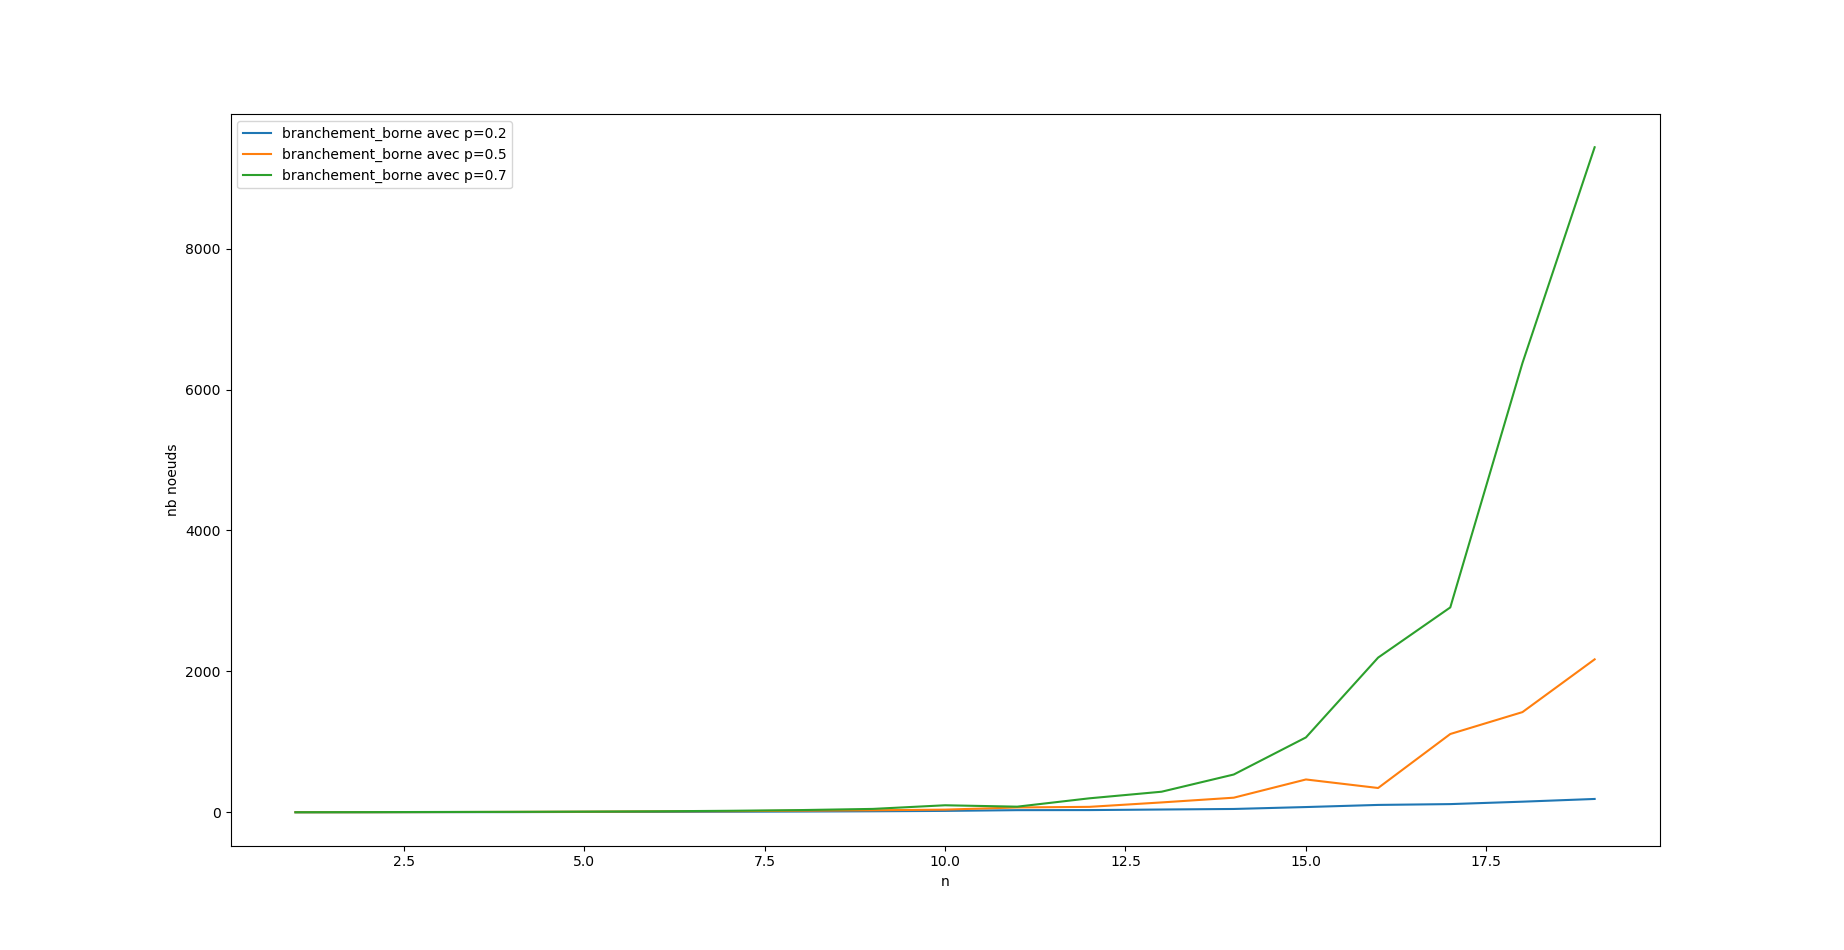
\includegraphics[scale=0.3]{"./test_nb_noeuds_branchement_borne.png"}

Q4.2.3 : 
Voilà une graphique permettant de tester le temps d'execution avec l'algorithme glouton pour sélectionner quelle branche on visite en premier. On constate que l'algorithme glouton est trop long à s'executer par rapport au temps qu'il fait gagner... Cette méthode n'est donc pas rentable.

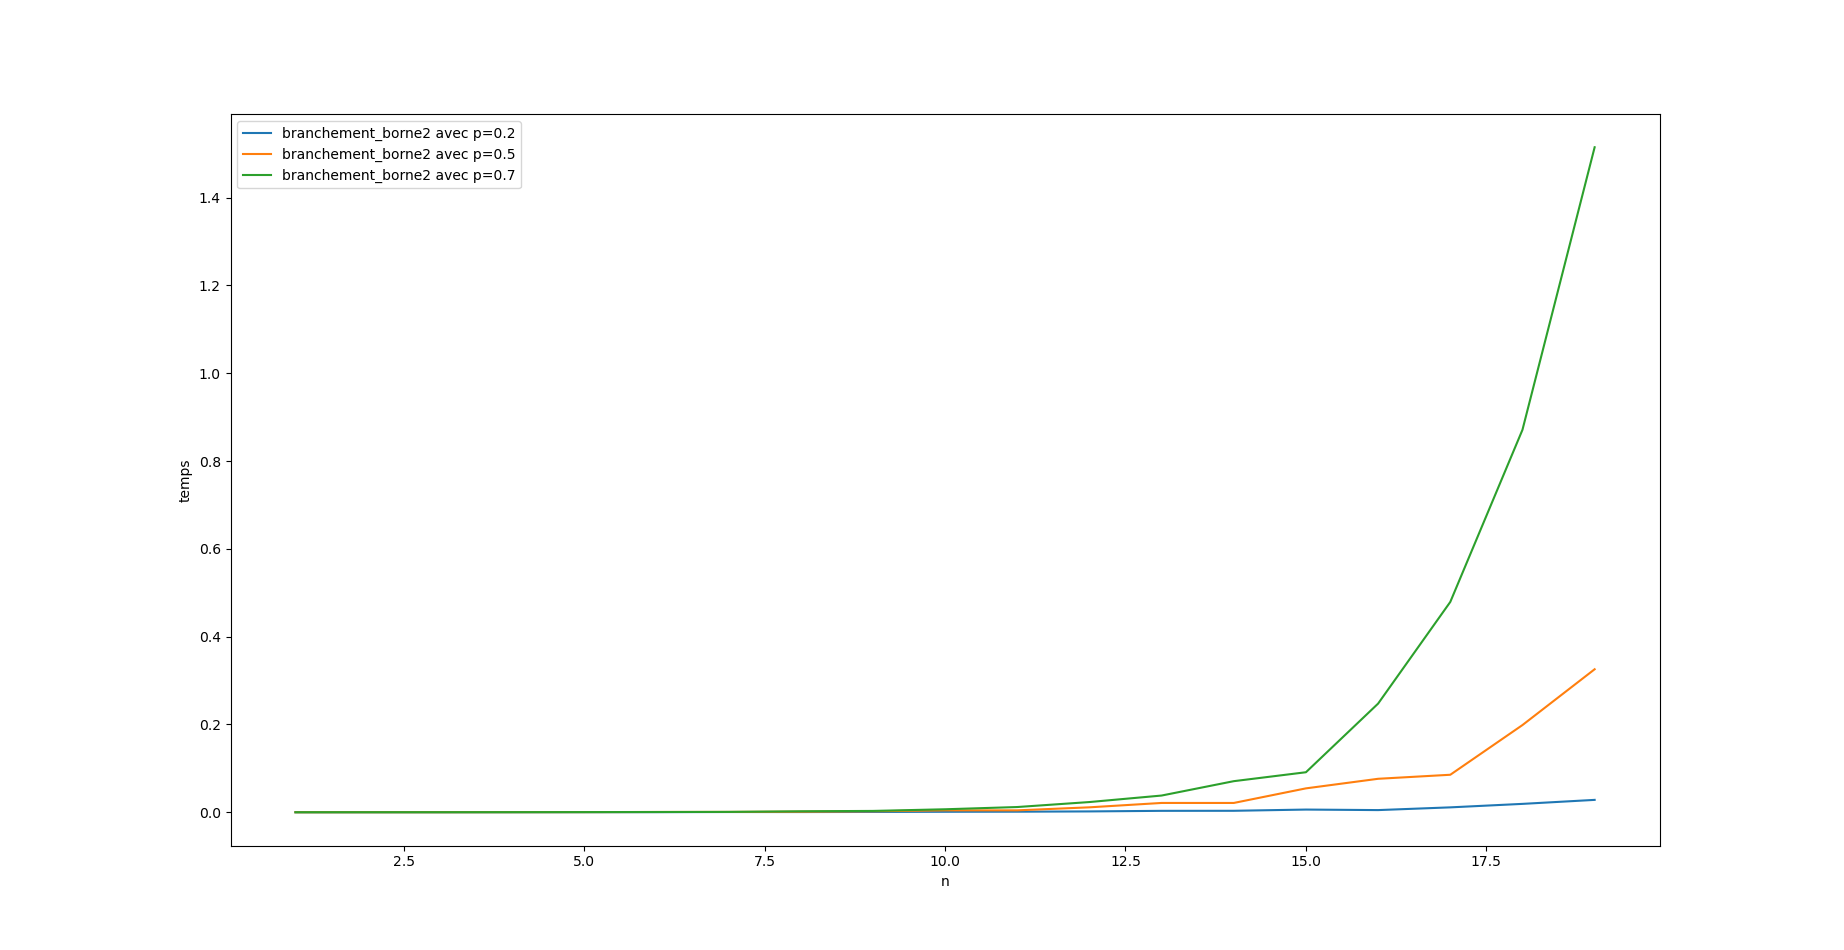
\includegraphics[scale=0.3]{"./test_branchement_borne2.png"}

Voilà une graphique permettant de tester le temps d'execution avec l'algorithme glouton pour sélectionner quelle branche on visite en premier et en retirant les bornes inférieures. C'est encore pire !

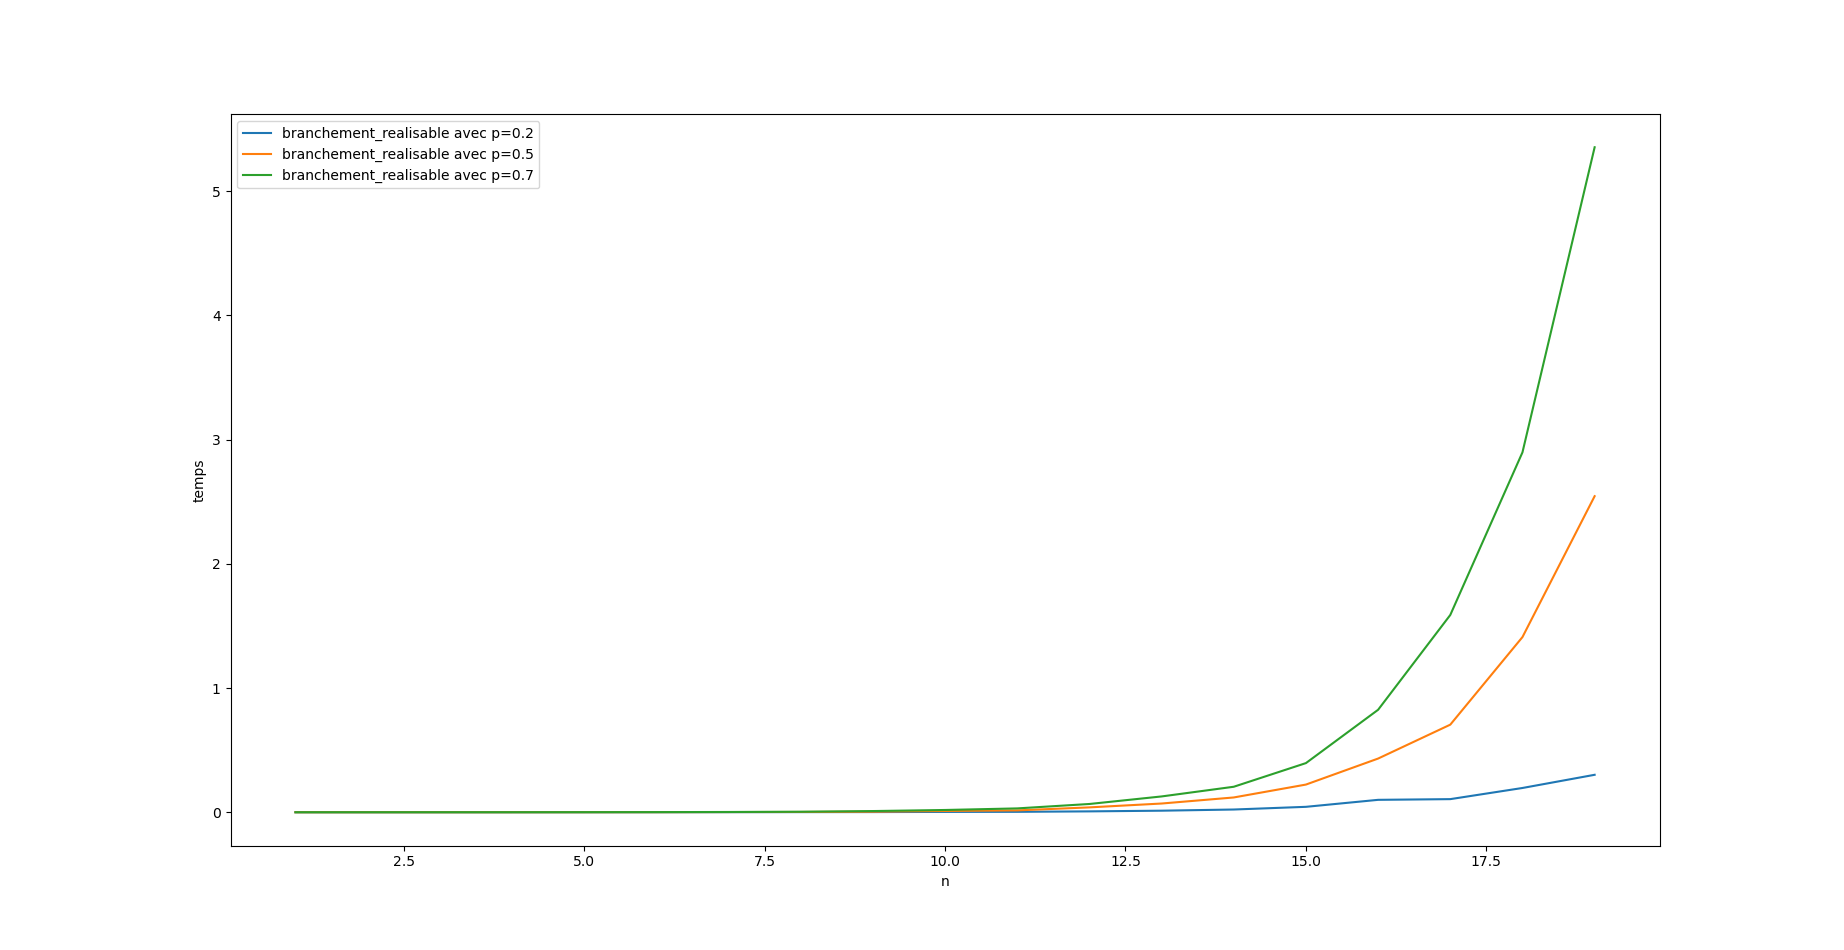
\includegraphics[scale=0.3]{"./test_branchement_realisable.png"}

Q4.3.1 : 
Le branchement amélioré fait gagner beaucoup de temps et de noeuds visités !

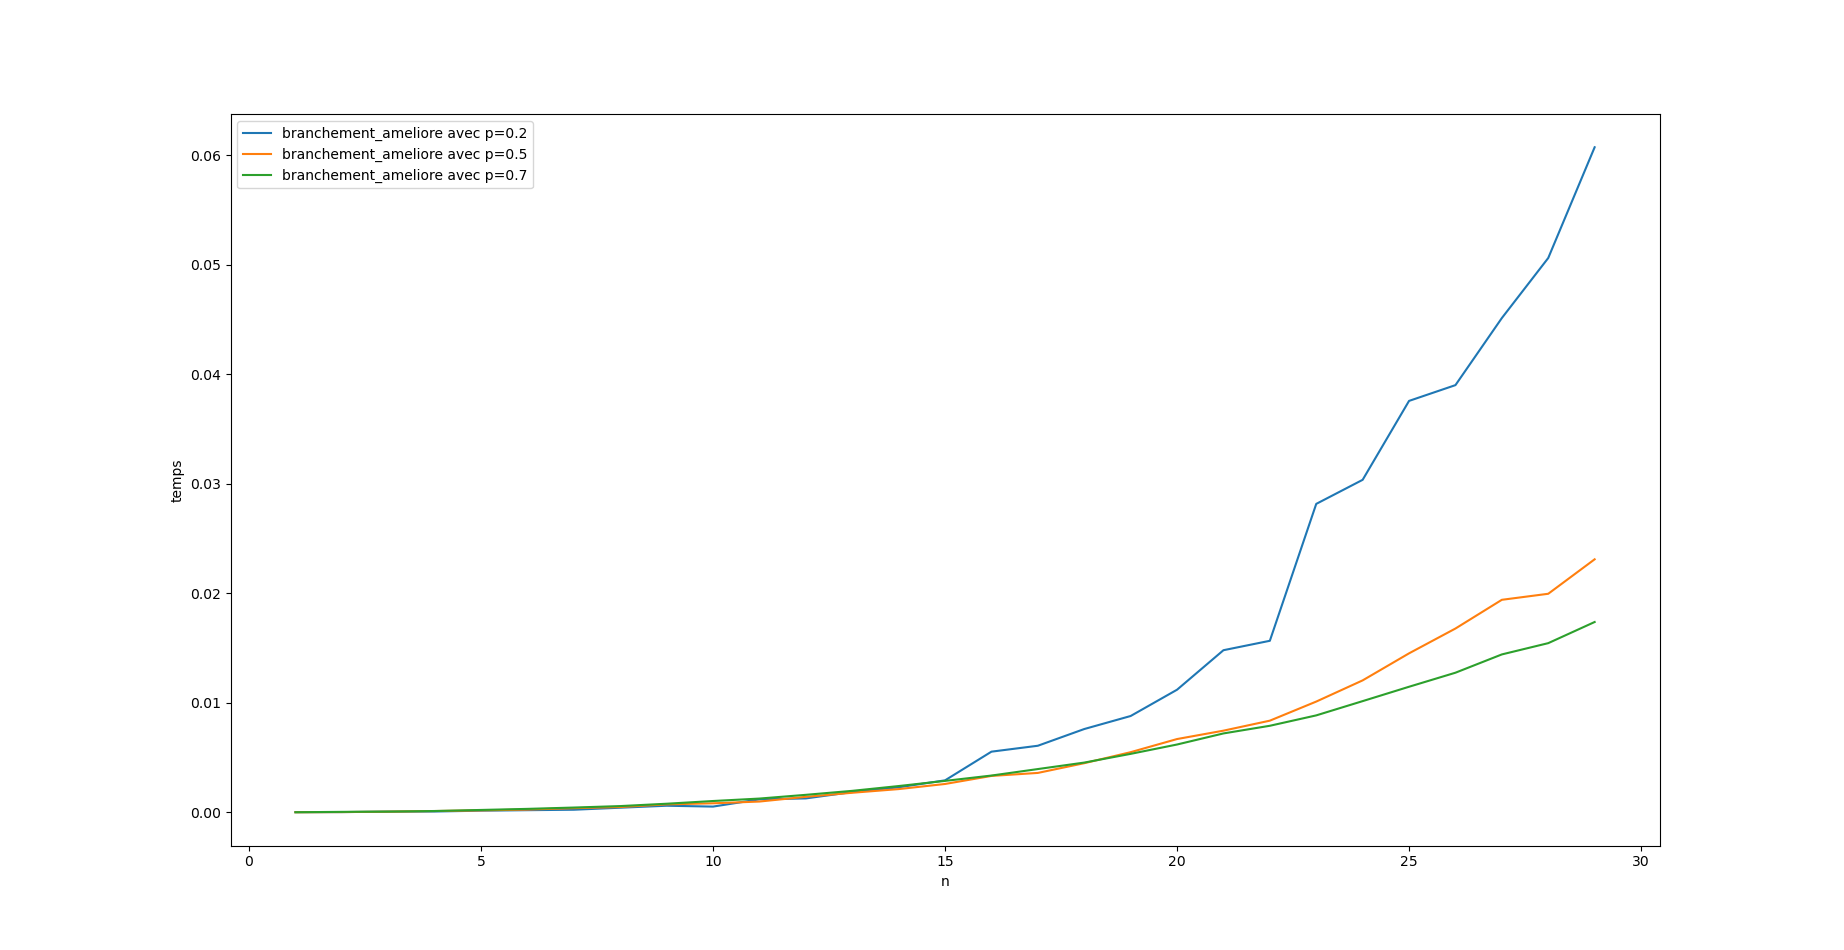
\includegraphics[scale=0.3]{"./test_branchement_ameliore.png"}
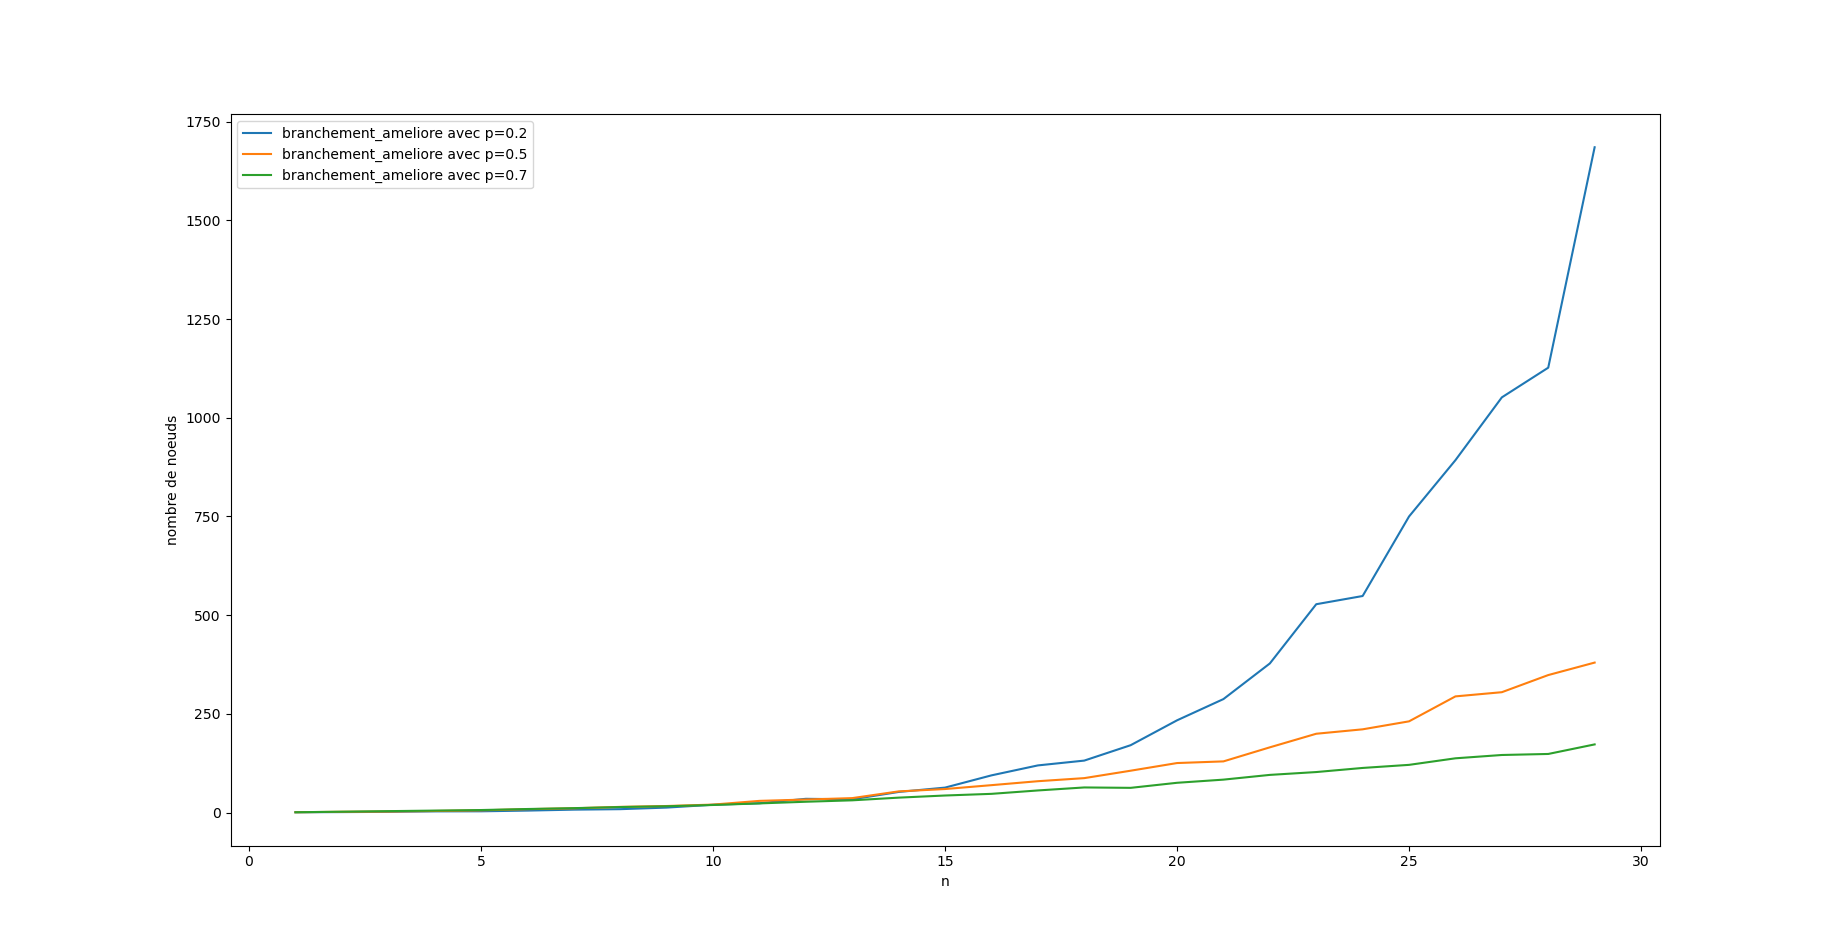
\includegraphics[scale=0.3]{"./test_nombre_noeuds_branchement_ameliore.png"}

Q4.3.3 :
Soit $G$ un graphe et $C$ un couverture minimale de $G$ ainsi que $s$ un sommet de degré 1 de $G$. Si $s \in C$, notons $v$ l'unique voisin de $s$ qui n'est pas dans $C$ (il existe sinon $C\textbackslash\{s\}$ est une couverture de taille strictement inférieure à $C$). Alors $(C\textbackslash\{s\}) \cup \{v\}$ est une couverture de $G$ qui ne contient pas $s$. Ainsi pour tout sommet $s$ de degré 1, il existe une couverture qui ne contient pas $s$. \\

Q4.4.1 : 
Voilà des graphiques permettant de comparer les rapports d'approximation de l'algorithme glouton et de l'algorithme de couplage. Le pire rapport pour l'algorithme de couplage est 1,8 et le pire rapport pour l'algorithme glouton est 0,9.

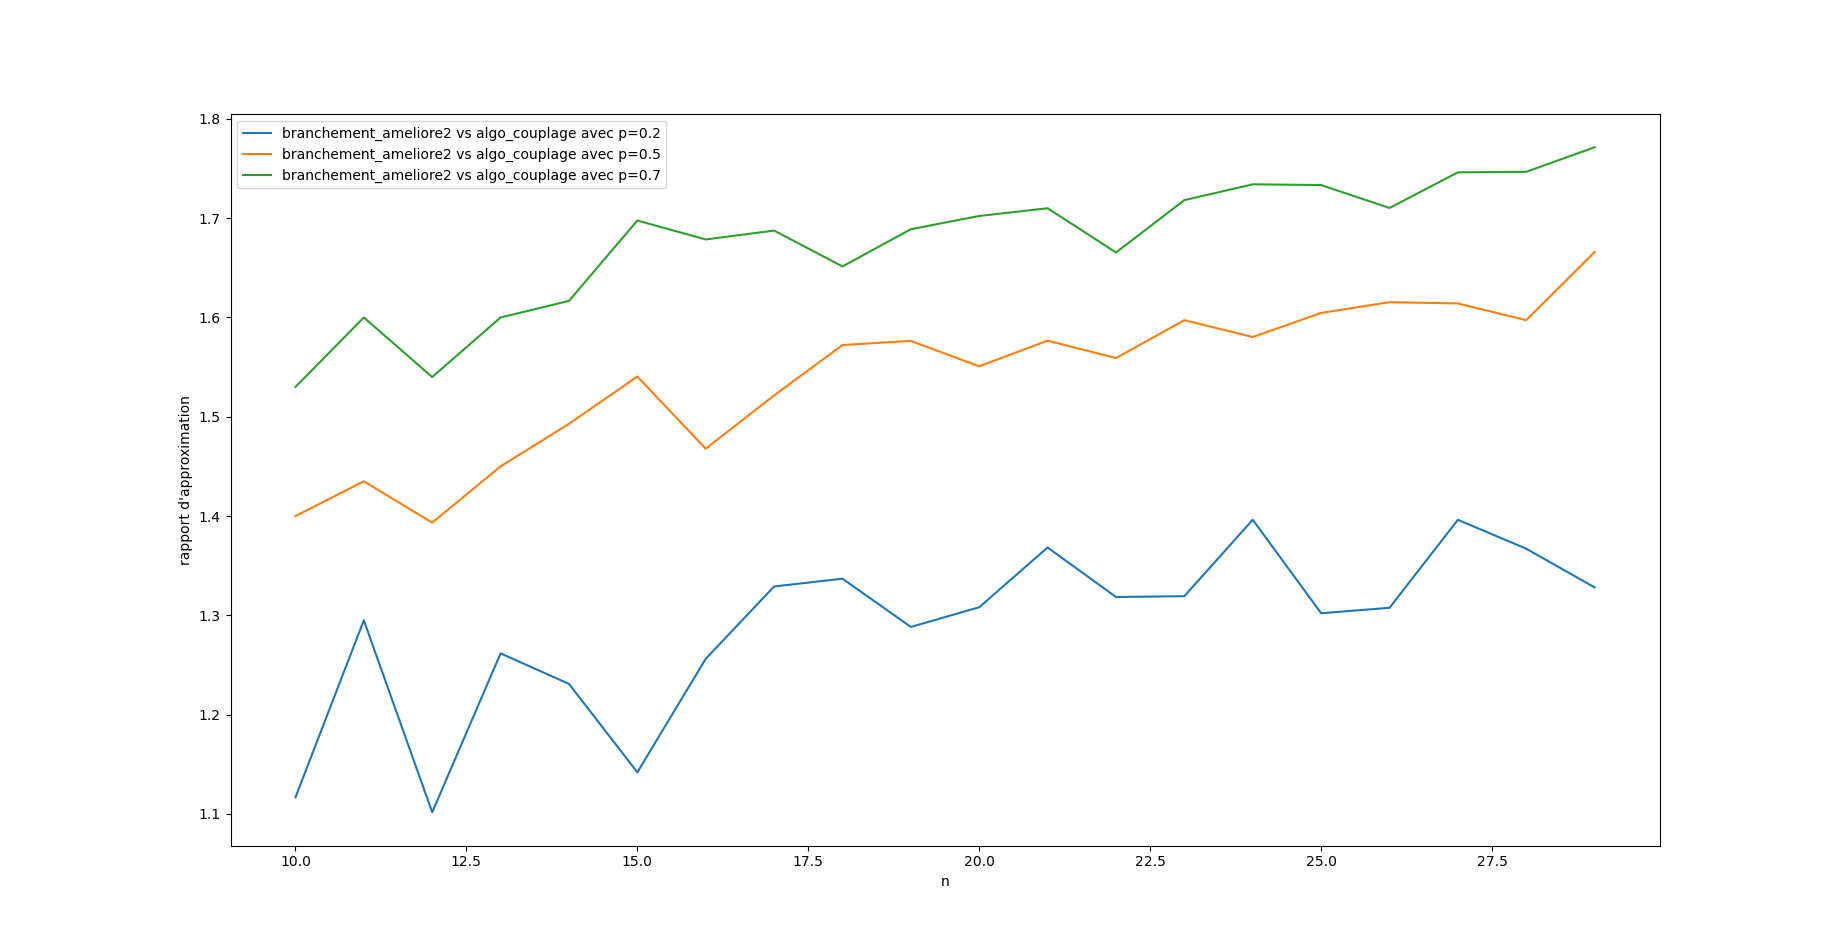
\includegraphics[scale=0.3]{"./rapport_approx_couplage.png"}
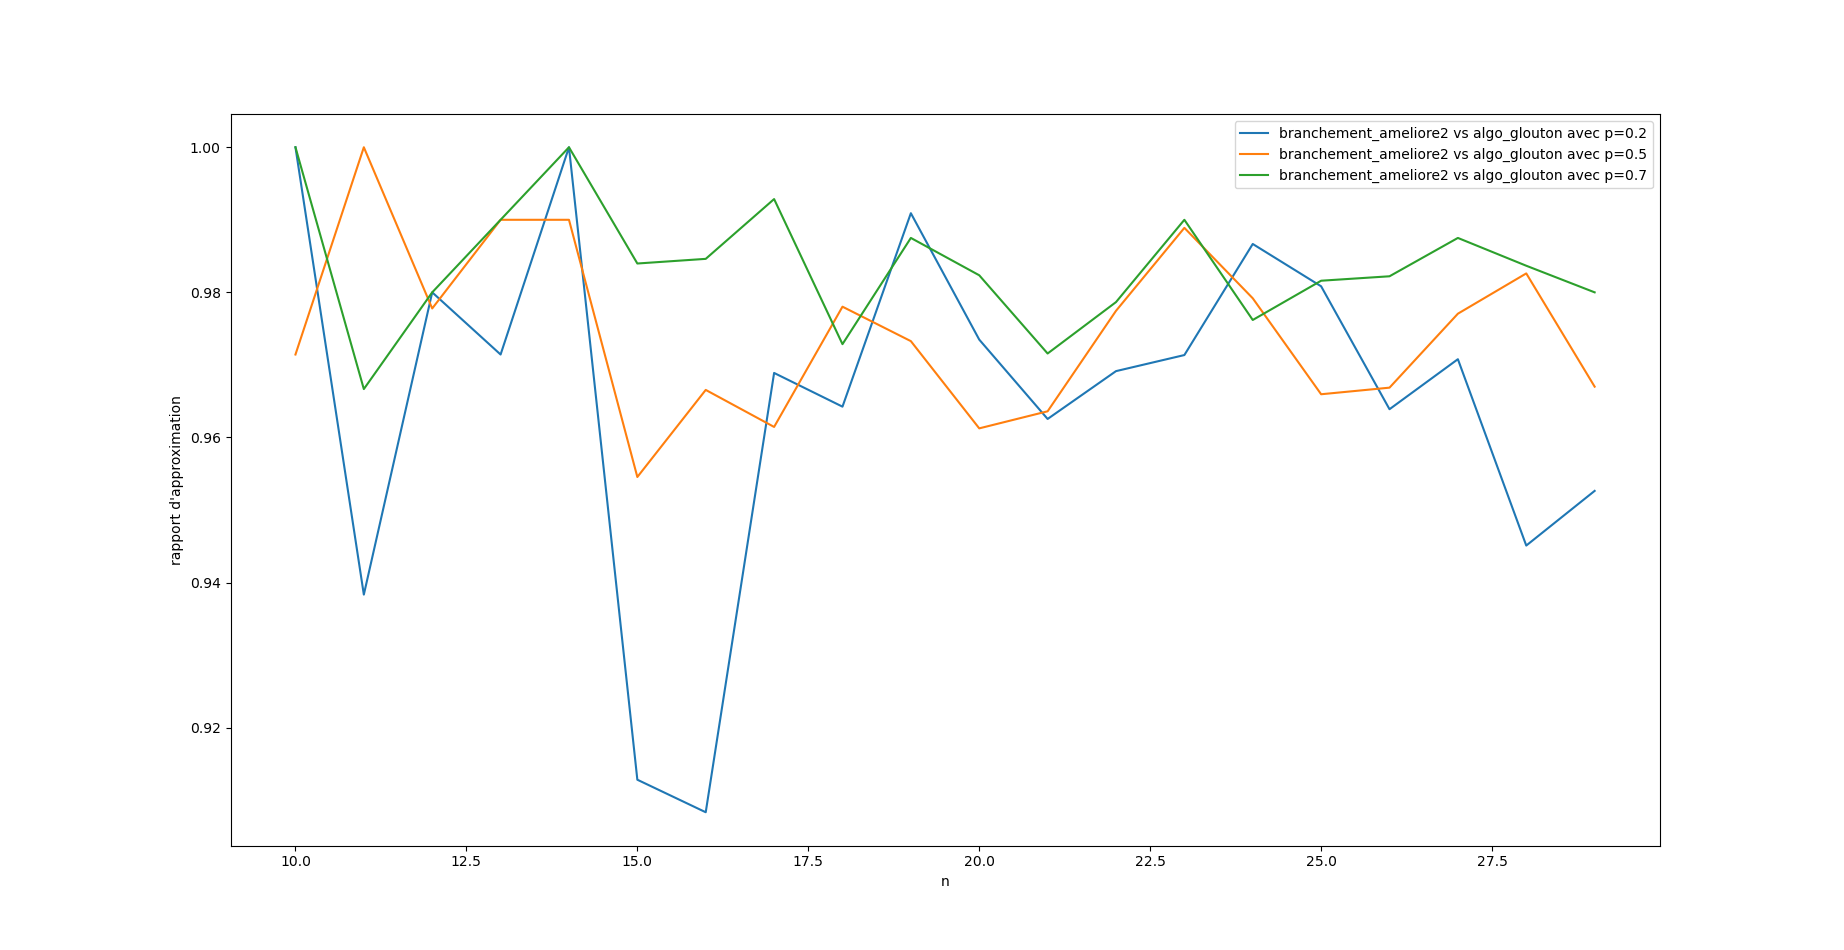
\includegraphics[scale=0.3]{"./rapport_approx_glouton.png"}

\end{document}
